\chapter{Results and Discussion}\label{chapter:results}

This chapter shows the evaluation results of for the two different machine learning models on different subcorpora, namely, abstracts and full text.

\section{Results for \textit{SSModel} on Abstracts Subcorpus}

This section presents the results for same-sentence model (\textit{SSModel}) on the LocText abstracts subcorpus. The results are initially discussed for the model trained on training data and evaluated on development data. All experimentation such as feature selection or hyperparameter search is performed with the development data. Once the number of features to keep are fixed and the hyperparameter is exhaustively searched, the training model is evaluated on the test data. The results on unseen test data are considered final results. All following subsections until subsection \ref{subsec:SSFinalRes} presents the results for a model trained on training data and evaluated on development data.

%After all experimentation, an additional model is training combining training and development data. Such a model is used to evaluate the test data and the results in such a way are considered much more robust.

\subsection{Initial Results}

\begin{figure}
\centering
\begin{minipage}{.5\textwidth}
  \centering
  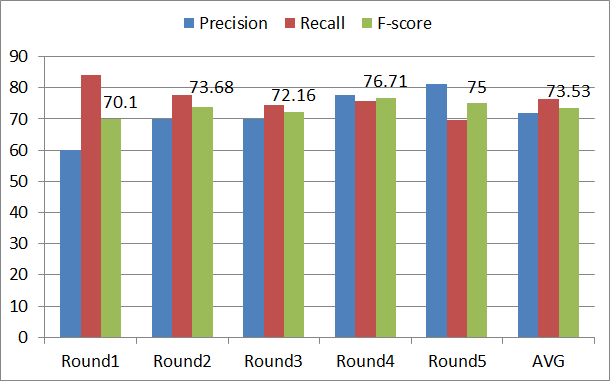
\includegraphics[width=.95\textwidth]{figures/SSInitialResultsNUniq.png}
  \caption{\textit{SSModel}, non unique, initial.}
  \label{fig:SS_NU_Initial}
\end{minipage}%
\begin{minipage}{.5\textwidth}
  \centering
  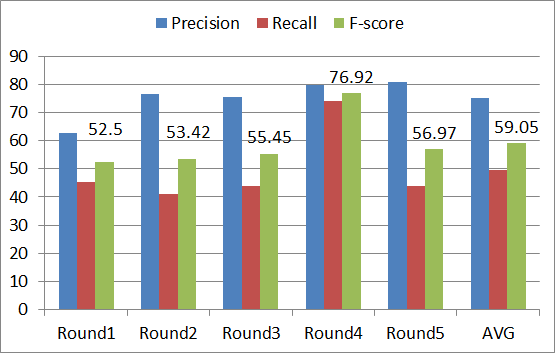
\includegraphics[width=.95\textwidth]{figures/SSInitialResultsUniq.png}
  \caption{\textit{SSModel}, unique, initial.}
  \label{fig:SS_U_Initial}
\end{minipage}
\end{figure}

As explained in Section \ref{sec:training}, 5-fold cross-validation is performed on the LocText corpus. The initial evaluation results are shown in figures \ref{fig:SS_NU_Initial} and \ref{fig:SS_U_Initial}. Figure \ref{fig:SS_NU_Initial} shows the results of \textit{SSModel} using non unique evaluation mode (Section \ref{subsubsec:NonUniqEval}) and Fig. \ref{fig:SS_U_Initial} shows the results of \textit{SSModel} using unique evaluation mode (Section \ref{subsubsec:UniqEval}). The results are shown in terms of \textit{Precision} (\ref{subsubsec:Prec}), \textit{Recall} (\ref{subsubsec:Recal}) and \textit{F score} (\ref{subsubsec:Fscore}) for every round of cross validation the performance is averaged in the end. The \textit{F score} bars in the figures are also labeled with the actual value. The non unique average \textit{F score} for \textit{SSModel} is 73.53 and the unique average \textit{F score} for \textit{SSModel} is 59.05.

\subsubsection{Feature Selection}

In order to make \textit{SSModel} robust and adaptable to other corpora, several experiments were carried out. Every round of cross validation creates a model from around 30000 features on average. Many of these features can be very specific to the LocText corpus and therefore, efforts are directed to discard unnecessary and overfitting features. Following feature selection methods were tried:

\begin{itemize}

\item Leave-One-Out Analysis
\item Feature Weight Ranking
\item Information Gain Analysis

\end{itemize}

These methods are discussed in the following sections.

\subsection{Results after Leave-One-Out Analysis}

\begin{figure}
\centering
\begin{minipage}{.5\textwidth}
  \centering
  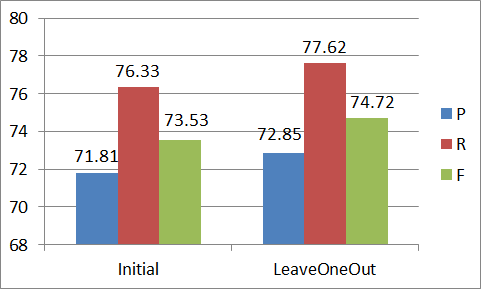
\includegraphics[width=.95\textwidth]{figures/LeaveOneOutNUniq.png}
  \caption{\textit{SSModel}, non u., LeaveOneOut.}
  \label{fig:LeaveOO_NU}
\end{minipage}%
\begin{minipage}{.5\textwidth}
  \centering
  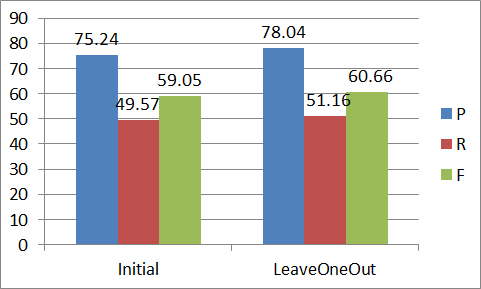
\includegraphics[width=.95\textwidth]{figures/LeaveOneOutUniq.png}
  \caption{\textit{SSModel}, uniq., LeaveOneOut.}
  \label{fig:LeaveOO_U}
\end{minipage}
\end{figure}

The theoretical aspects of Leave-One-Out approach are discussed in detail in Subsection \ref{subsec:LeaveOneOut}. To summarize this approach, the feature generators or functions that yield the lowest performances are greedily discarded.

Figure \ref{fig:LeaveOO_NU} and \ref{fig:LeaveOO_U} show the comparison between the results of the initial model and after performing the \emph{LeaveOneOut} experimentation.  The \textit{Precision}, \textit{Recall} and \textit{F score} are denoted by P, R and F respectively. Figure \ref{fig:LeaveOO_NU} shows the comparison using non-unique evaluation mode and \ref{fig:LeaveOO_U} shows the comparison using unique evaluation mode. As shown in the figures, the average \textit{F score} increased from 73.53 to 74.72 for non-unique evaluation and from 59.05 to 60.66 for unique evaluation. In addition to the increase in the performance, the average number of features was slightly reduced. The initial model used around 30900 features on average in every round of the cross validation whereas the model refined after \emph{LeaveOneOut} experimentation uses 29000 features on average in every round, therefore reducing the number of features by 1900 for every round of the cross-validation.

\subsection{Results after Feature Weight Ranking}

The Feature Weight Ranking (FWR) approach, discussed in detail in Subsection \ref{subsec:FWR}, uses the weights of the features for feature selection. Support vector machines (SVMs), while creating a hyperplane to separate positive and negative instances in the training data, learns the weights for the features. These weights can be extracted from the learned model using a perl script \cite{svmlightonline}.


\begin{figure}
\centering
\begin{minipage}{.5\textwidth}
  \centering
  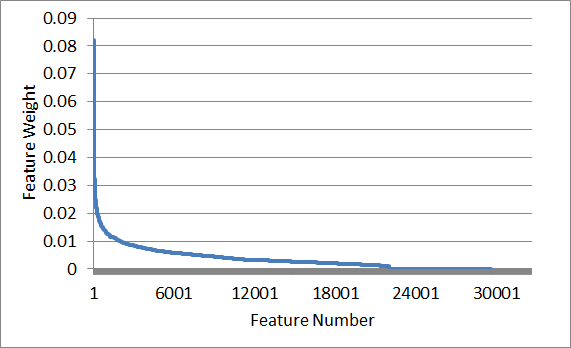
\includegraphics[width=.95\textwidth]{figures/FWRWeightDist.png}
  \caption{Feature weight distribution.}
  \label{fig:FWRWeightDist}
\end{minipage}%
\begin{minipage}{.5\textwidth}
  \centering
  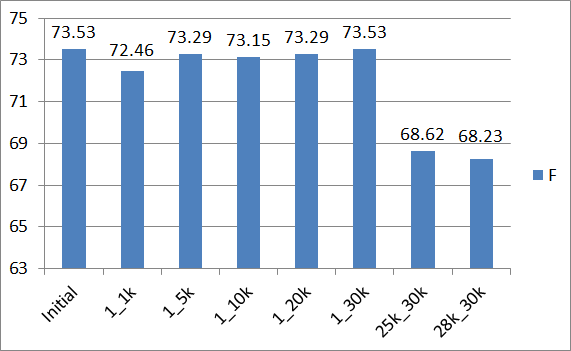
\includegraphics[width=.95\textwidth]{figures/FWRPerformance.png}
  \caption{FWR Performance comparison.}
  \label{fig:FWRPerfComp}
\end{minipage}
\end{figure}

For each round of cross-validation, a model is learned and therefore, the feature weights can be extracted for every round. Figure \ref{fig:FWRWeightDist} shows the distribution of weights for features of round 1, from highest weighted feature to lowest weighted feature. The weights of the features in other folds follow a similar distribution. As shown in the figure, there are very less features with higher weights and most of the features have comparatively lower weights.

Figure \ref{fig:FWRPerfComp} shows the comparison of performance of various FWR (Feature Weight Ranking) models with the initial model. Only average \textit{F scores} are shown for comparison. The model \textit{1\_1k} implies that the model is trained using 1000 highest weighted features from every round of cross validation. Similar terminology applies for the rest of the FWR models shown in the figure. None of the FWR models have a higher performance than the initial model. The performance of the FWR model with first 1000 features (\textit{1\_1k}) is lower than the FWR model with first 5000 features (\textit{1\_5k}). It can also be seen that the performance drops for first 10000 (\textit{1\_10k}) features and then again increases for 20000 (\textit{1\_20k}) and 30000 (\textit{1\_30k}) features. This trend invalidates the intuition that higher-weighted features should result in higher performance and adding lower-weighted features should decrease the performance. In our case, adding features ranked 10000 to 20000 actually increased the performance. The FWR model consisting of the lowest 2000 features in every round (\textit{28k\_30k}) also has considerable performance and cannot be discarded as useless. Owing to all these problems, this feature selection approach was not further experimented.

\subsection{Results after Information Gain Analysis}\label{subsec:SS_IG}

Information gain (IG) is widely for feature selection. The theoretical background for calculating IG can be found in Subsection \ref{subsec:IG}. The features' IG is calculated in every round of cross validation.

\begin{figure}
\centering
\begin{minipage}{.5\textwidth}
  \centering
  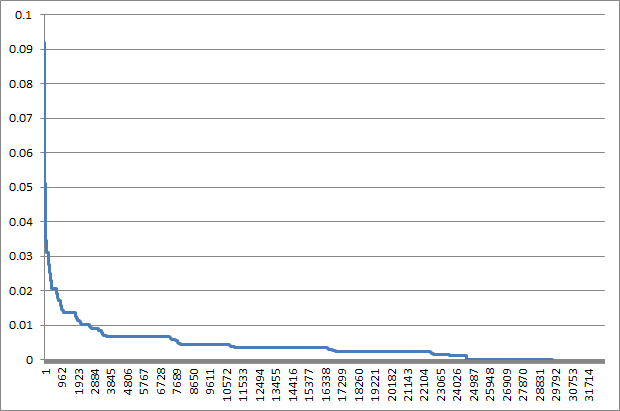
\includegraphics[width=.95\textwidth]{figures/IGDistr1.png}
  \caption{IG distribution.}
  \label{fig:IGDist}
\end{minipage}%
\begin{minipage}{.5\textwidth}
  \centering
  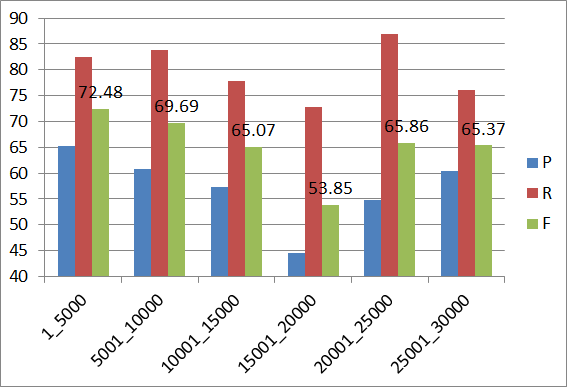
\includegraphics[width=.95\textwidth]{figures/IG5kSlabsComp.png}
  \caption{IG models with 5k chunks.}
  \label{fig:IG5kComp}
\end{minipage}
\end{figure}

Figure \ref{fig:IGDist} shows the IG of the features used in round 1. The distribution of IG is somewhat similar to the distribution of feature weights. However, the feature weight distribution is smoother than the distribution of IG. To analyze the effectiveness of features with different IG, an experiment was conducted by dividing the features into chunks of 5000 features depending on their IG. Figure \ref{fig:IG5kComp} shows the average performance of various models trained with chunks of 5000 features. The model \textit{1\_5000} uses the first 5000 features with best IG, the model \textit{5001\_10000} uses next 5000 features and so on. As seen in the figure, none of the 5k models have exceptionally low performance except model \textit{15001\_20000}. This further consolidates the finding of Joachims et al. \cite{joachims1998text} that all features have some or other information and aggressive feature selection might not result in manifold increase in the performance.

Further experiments were carried out using some of the features with best IG. For this purpose, the first 5000 features were considered. Different models were trained using the first 1000, 2000, 4000 and 5000 features and their performance was compared with the initial model. Figure \ref{fig:IG_5k_NU} shows the models comparison using non unique evaluation mode and \ref{fig:IG_5k_U} shows the models comparison using unique evaluation mode. As seen in Fig. \ref{fig:IG_5k_U}, the model with the first 2000 features registers much better performance than the initial model. For the same model, the non unique comparison in Fig. \ref{fig:IG_5k_NU} shows highest the increase in \textit{Recall}, from 73.83 to 84.74.

\begin{figure}
\centering
\begin{minipage}{.5\textwidth}
  \centering
  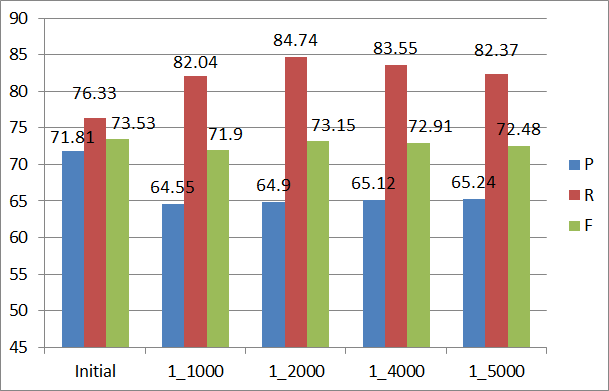
\includegraphics[width=.95\textwidth]{figures/IGFirst5k_NU.png}
  \caption{IG non unique comparison.}
  \label{fig:IG_5k_NU}
\end{minipage}%
\begin{minipage}{.5\textwidth}
  \centering
  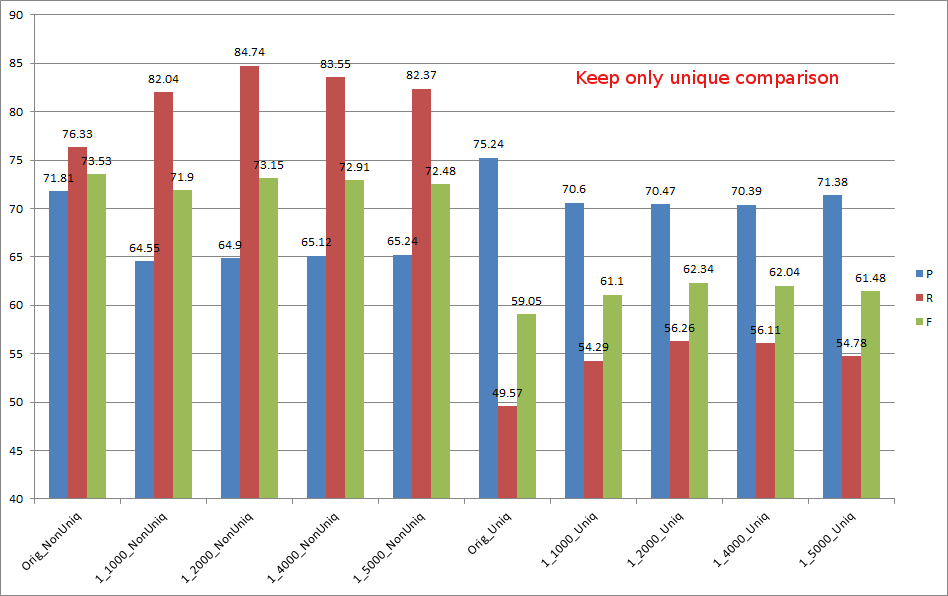
\includegraphics[width=.95\textwidth]{figures/IGFirst5k_U.png}
  \caption{IG unique comparison.}
  \label{fig:IG_5k_U}
\end{minipage}
\end{figure}


As previously described, the features are generated by feature generators or functions. Note that the terms ``feature generator'' and ``feature function'' mean the same and are used interchangeably in the explanation ahead. In order to discard bad features, the solution is to discard the feature generators that decrease performance. A feature generator can generate many features and the option is to either keep all of them or discard all of them. Hence, it was necessary to trace back the feature generators from the features. Once the feature generators are located, other features generators can be discarded and the performance of such a model can be observed.

To trace back the feature generators, every feature was given a label indicating the feature generator that produced it. There were a total of 109 feature generators and to choose some of them, it was necessary to assign a count to each feature generator. Following criteria were used for the selection of feature generators:

\begin{itemize}

\item \textbf{Total IG (TIG):} for every feature generator, the IG of its features in all 5 rounds of cross validation was summed up to produce a number called total IG or TIG.

\item \textbf{Number of features:} the number of features produced by each feature generator.

\item \textbf{Average IG (AvgIG):} the average IG for a feature generator is equal to its TIG divided by its produced number of features.

\item \textbf{Minimum IG (MinIG):} the minimum IG for a feature generator is equal to the minimum IG of its features.

\item \textbf{Maximum IG (MaxIG):} the maximum IG for a feature generator is equal to the maximum IG of its features.

\end{itemize}

Using these 5 criteria, an exhaustive search was conducted to select the best model. For every criterion, a model was trained and evaluated using some or all of the 109 feature generators. For instance for TIG, the models were named as $TIG_{1}$ to $TIG_{109}$. $TIG_{1}$ denotes a model with a single feature generator with the best TIG. Similarly, $TIG_{10}$ denotes a model trained using the 10 feature generators with highest TIG. Such experiments were conducted for all of the 5 criteria/statistics mentioned above. By far, the best results were obtained with AvgIG and MinIG.

\begin{figure}
\centering
\begin{minipage}{.5\textwidth}
  \centering
  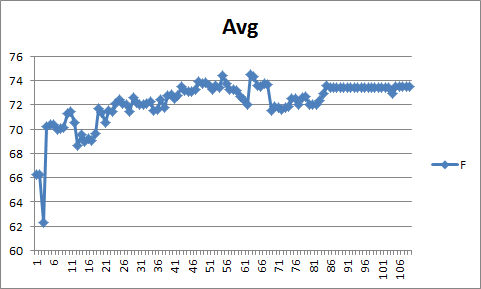
\includegraphics[width=.95\textwidth]{figures/AvgIGAnalysis.png}
  \caption{AvgIG models' scores.}
  \label{fig:AvgIG}
\end{minipage}%
\begin{minipage}{.5\textwidth}
  \centering
  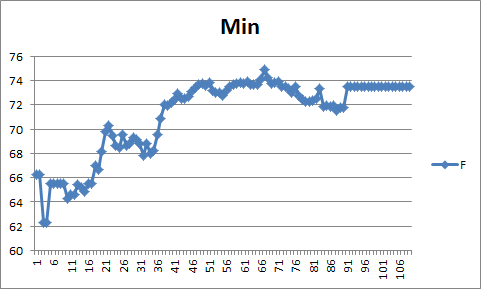
\includegraphics[width=.95\textwidth]{figures/MinIGAnalysis.png}
  \caption{MinIG models' scores.}
  \label{fig:MinIG}
\end{minipage}
\end{figure}

Figures \ref{fig:AvgIG} and \ref{fig:MinIG} show the variation of \textit{F scores} of different models created AvgIG and MinIG, respectively. For AvgIG, the models are addressed as $Avg_1$ to $Avg_{109}$ depending on the number of feature generators used for training. Similarly, for MinIG, the models are addressed as $Min_{1}$ to $Min_{109}$. The last score and point in the graph line $Avg_{109}$ or $Min_{109}$ shows the performance of the respective model using all 109 feature generators, i.e., without any feature selection. Thus, the performance of $Avg_{109}$ and $Min_{109}$ is equal to the performance of initial model, which is \textit{F score} of 73.53 according to the non unique evaluation method. In Fig. \ref{fig:AvgIG}, three models, viz., $Avg_{55}$, $Avg_{63}$ and $Avg_{64}$ that have better performance than the initial model ($Avg_{109}$). Similarly, in Figure \ref{fig:MinIG}, there are three models, viz., $Min_{66}$, $Min_{67}$ and $Min_{68}$ that have better performance than the initial model ($Min_{109}$). These 6 models further analyzed.

\begin{figure}
\centering
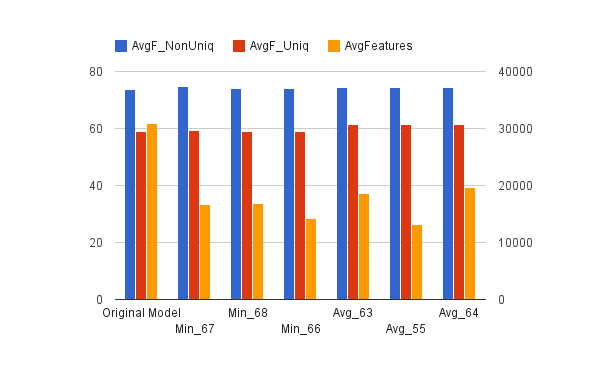
\includegraphics[scale=0.6]{figures/6ModelsComparison.png}
\caption{Comparison of selected models with initial model.}\label{fig:6ModelsComp}
\end{figure}

As shown in Fig. \ref{fig:6ModelsComp}, $Avg_{55}$ has near to best performance with respect to non unique evaluation mode, best performance with respect to unique evaluation mode and the highest reduction in the number of features. The average number of feature for $Avg_{55}$ is around 13230 compared to 30900 in the initial model. Therefore, the $Avg_{55}$ model was selected as the best \textit{SSModel}.


\subsection{Hyperparameter Search Results}

Exhaustive hyperparameter search was conducted for the selected model $Avg_{55}$. The hyperparameter for SVMs is the regularization parameter $\mathbf{C}$, which determines the trade-off between training error and test error as explained in Subsection \ref{subsec:RegPar}. Experiments were conducted for finding the best regularization parameter by varying $\mathbf{C}$ from 0.0000 to 2.0000 with steps of 0.0005. The value of 0.0005 was found to be the best hyperparameter value, which results in a performance increase of 1.76 points with respect to the unique evaluation mode. Note that the hyperparameter search was done to maximize the performance with respect to the unique evaluation mode.

\begin{figure}
\centering
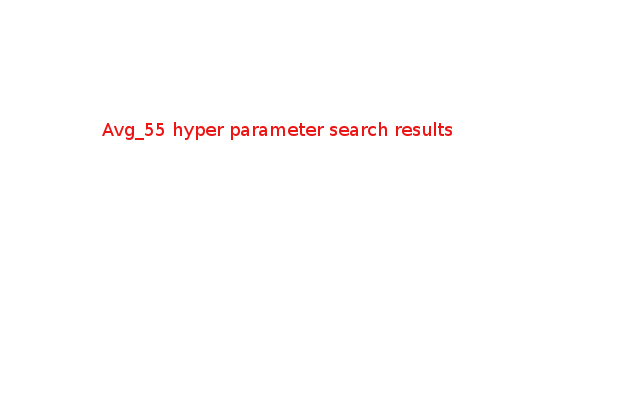
\includegraphics[scale=0.6]{figures/SSModelRegPar.png}
\caption{Performance results before and after feature selection and hyperparameter search on the development set for the unique mode evaluation.}\label{fig:SSModelRegPar} % j: TODO, reference this figure in the text
\end{figure}

\subsection{Final Results}\label{subsec:SSFinalRes}

\begin{figure}
\centering
\begin{minipage}{.5\textwidth}
  \centering
  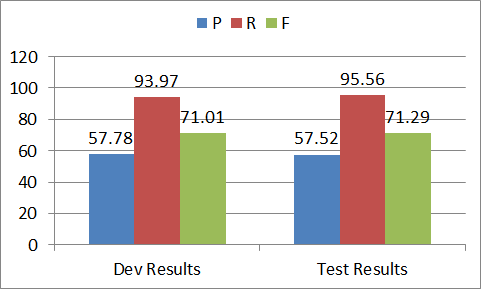
\includegraphics[width=.95\textwidth]{figures/CompDevTestResultsNonUniq.png}
  \caption{Non unique mode results.}
  \label{fig:SS_DevTest_NU}
\end{minipage}%
\begin{minipage}{.5\textwidth}
  \centering
  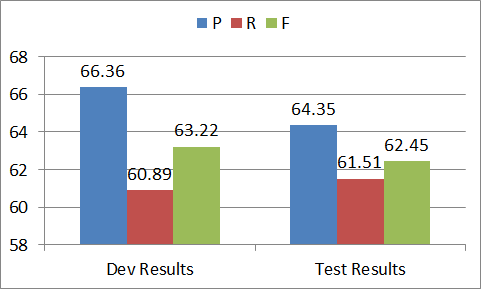
\includegraphics[width=.95\textwidth]{figures/CompDevTestResultsUniq.png}
  \caption{Unique mode results.}
  \label{fig:SS_DevTest_U}
\end{minipage}
\end{figure}

The optimal \textit{SSModel} trained after feature selection and hyperparameter search is finally evaluated on unseen test data. Since the test data is not touched during the tuning of the model, the evaluation on test data is considered a robust estimate of the model performance and hence, can be termed as final results for \textit{SSModel}.

Figure \ref{fig:SS_DevTest_NU} shows the comparison between average results of the optimal \textit{SSModel} on development set termed as "Dev Results" and test set termed as "Test Results". The results in Fig. \ref{fig:SS_DevTest_NU} are computed using non unique mode of evaluation. As shown in figure, the evaluation performance on the test set is nearly equal to the evaluation performance on the development set. While the average \textit{F score} for evaluation on development set is 71.01, the average \textit{F score} for evaluation on the test set is 71.29.

Figure \ref{fig:SS_DevTest_U} shows a similar comparison between the performance on the development set and the test set, but using unique mode of evaluation. Similar to the trends in Fig. \ref{fig:SS_DevTest_NU}, the evaluation performance on the test set is nearly equal to the evaluation performance on development set. As shown in the figure, the average \textit{F score} for evaluation on development set is 63.22, whereas the average \textit{F score} for evaluation on the test set is 62.45.

\section{Results for \textit{DSModel} on Abstracts Subcorpus}

This section discusses the evaluation of performance of the different-sentence model (\textit{DSModel}) on the abstracts subcorpus. The goal of the \textit{DSModel} is to extract the protein-location relations in which either of the entity is present in a different sentence. The overall objective of using two different models, viz. \textit{SSModel} and \textit{DSModel} is to extract as many protein-location relations from a whole document as possible.

The evaluation of performance of the \textit{DSModel} is, in a way, dependent on the predictions of the \textit{SSModel}. If unique mode of evaluation (Section \ref{subsubsec:UniqEval}) is considered, then it may happen that a particular relation predicted by the \textit{DSModel} is already predicted by the \textit{SSModel}. In this particular case, the \textit{DSModel} is not adding any extra information to the set of predictions. Therefore, utmost care is taken while evaluating the results of the \textit{DSModel}. Several evaluation criteria are developed to understand how the \textit{DSModel} is supplementing the set of predictions. These evaluation criteria are:

\begin{itemize}

\item \textit{SVM Performance:} this evaluation describes the performance of the SVM model. This is exactly the same as non unique mode of the evaluation (Subsection \ref{subsubsec:NonUniqEval}).

\item \textit{Unique performance:} this evaluation compares the set of predictions of the \textit{DSModel} with the unique set of relations for the document in the corpus. This is exactly the same as the unique mode of evaluation (Subsection \ref{subsubsec:UniqEval}).

\item \textit{Manipulated prediction:} in this evaluation mode, the predictions of the \textit{DSModel} are manipulated to some extent. The intuition behind this manipulation is, if a relation is predicted positively by the \textit{SSModel} (in other words, the \textit{SSModel} predicts that the entities in the relation are related and present in the same sentence), then it is unlikely that the same entities could be related in a different-sentence relation or otherwise they would not add anything in unique evaluation mode. Therefore, if a relation predicted by the \textit{DSModel} is found in the list of positive predictions by \textit{SSModel}, then that particular relation prediction is manipulated into a negative prediction, irrespective of whether it was a positive prediction or a negative prediction earlier.

\item \textit{Combined evaluation:} The predictions of \textit{SSModel} and \textit{DSModel} are combined in a unique set of predictions. This also means that if a relation is predicted both by \textit{SSModel} and \textit{DSModel}, then the prediction is added to the unique set once. This unique set of predictions is then compared with the unique set of relations for every document in the corpus and the results are computed.

\end{itemize}

\subsection{Initial Results}

\begin{figure}
\centering
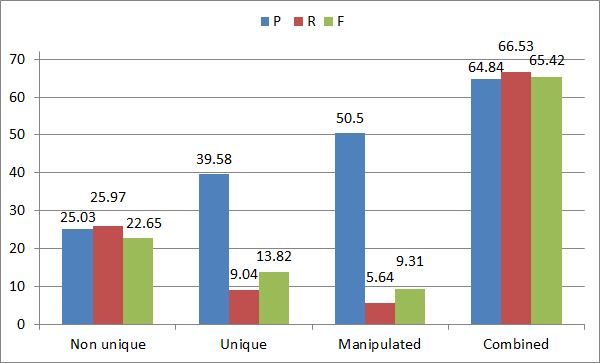
\includegraphics[scale=0.7]{figures/DSInitialResults.png}
\caption{Initial results of \textit{DSModel}.}\label{fig:DSInitial}
\end{figure}

Figure \ref{fig:DSInitial} shows the initial results of the \textit{DSModel}. These are the results prior to any experimentation for feature selection or hyperparameter search. The results are shown in the figure according to various evaluation criteria explained in the previous section. The original data, used for extraction of different-sentence relations, was totally imbalanced. The ratio of positive examples to negative examples was 1:10. It is difficult to train a model using such highly skewed data. Therefore, it was necessary to undersample \cite{akbani2004applying} the negative class to get some classification performance. The ratio of 1:5 was found optimal and all further experiments are carried out after undersampling the majority class (negative class).

For combined evaluation, the predictions of the \textit{DSModel} are combined with predictions of best performing \textit{SSModel}, i.e., the predictions generated by $Avg_{55}$ model trained using optimal hyperparameter.

\subsection{Optimizing Combined Evaluation}

During various experiments, it was found out that the non unique performance does not correlate well the with combined evaluation performance. In other words, if efforts are aimed to maximize non-unique or unique performance of the \textit{DSModel}, this does not necessarily optimize the combined performance of both \textit{SSModel} and \textit{DSModel}. This, for instance, may happen when the optimal \textit{DSModel} non-unique performance produces more repeated predictions that are already predicted by the \textit{SSModel}. Therefore, it was decided that efforts should be made to optimize the combined performance rather than unique or non-unique performance for the \textit{DSModel} alone.

Feature selection performed on the \textit{DSModel} is analogous to that of \textit{SSModel}'s. Three feature selection methods were tried, viz. Leave-One-Out Analysis, Feature Weight Ranking and Information Gain Analysis. Following subsections describe the results of these experiments.

\subsection{Results after Leave-One-Out Analysis}

The theoretical background for Leave-One-Out approach is discussed in Subsection \ref{subsec:LeaveOneOut}. In this approach, the feature generators or functions are greedily discarded to produce the best possible performance.

\begin{figure}
\centering
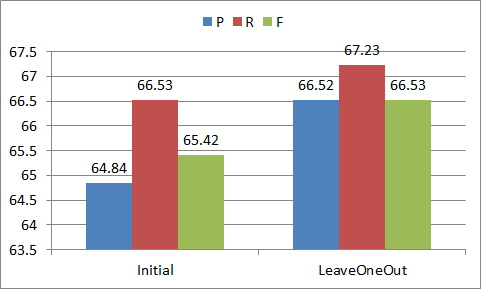
\includegraphics[scale=0.8]{figures/DSLeaveOneOutComb.png}
\caption{Effect of Leave-One-Out Analysis on \textit{DSModel}.}\label{fig:DSLeaveOO}
\end{figure}

Figure \ref{fig:DSLeaveOO} shows the effect of Leave-One-Out experimentation. The \textit{F score} for combined evaluation increased from 65.42 to 66.53. The total number of features used by initial model for 5 rounds of cross-validation was 310512 (62000 features per round of cross-validation on average). After Leave-One-Out experimentation, the total number of features for 5 rounds dropped to 201475 (average 40295 features per round), thereby reducing the number of features to a good extent.

\subsection{Results after Feature Weight Ranking}

The Feature Weight Ranking (FWR) approach is discussed in detail in Subsection \ref{subsec:FWR}. This approach uses the feature weights learned by Support Vector Machine (SVM), for the purpose of feature selection.

\begin{figure}
\centering
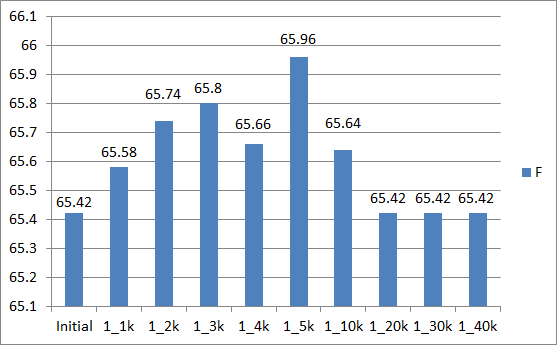
\includegraphics[scale=0.7]{figures/DSFWRResults.png}
\caption{Effect of Feature Weight Ranking approach on \textit{DSModel}.}\label{fig:DSFWR}
\end{figure}

Figure \ref{fig:DSFWR} shows the comparison between average \textit{F score} for combined evaluation mode. Initial model shows the performance before any experimentation. The model 1\_1k implies that 1000 highest weighted features from every round of cross validation are used for training the model. Similarly, the model 1\_20k implies that 20000 highest weighted features from every round of cross validation are used for training the model. As shown in Fig. \ref{fig:DSFWR}, the model 1\_5k register the best performance. However, the performance obtained is lower than the best performance obtained by LeaveOneOut experimentation and therefore, this approach was not further investigated. The weights of the features followed similar distribution as followed by the weights of the features for \textit{SSModel} in Fig. \ref{fig:FWRWeightDist}.

\subsection{Results after Information Gain Analysis}


Information gain analysis is most widely used approach for the purpose of feature selection. The theoretical aspects of Information Gain Analysis are discussed in Subsection \ref{subsec:IG}. The approach is also widely discussed for SSModel in Subsection \ref{subsec:SS_IG}.

\begin{figure}
\centering
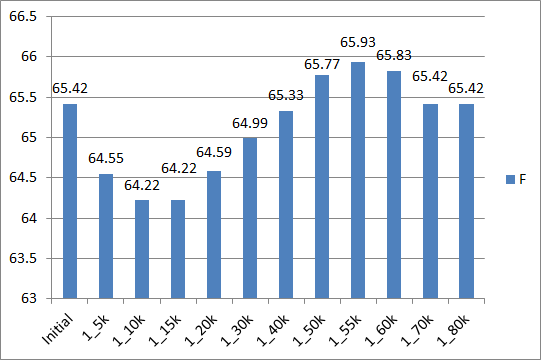
\includegraphics[scale=0.7]{figures/DSIGResults.png}
\caption{Effect of Information Gain Analysis on \textit{DSModel}.}\label{fig:DSIG}
\end{figure}


The initial model has close to 62000 average features for every round of cross validation. Information gain is calculated for every feature. The information gain for the features in every round follows similar distribution as observed in Fig. \ref{fig:IGDist}.

Figure \ref{fig:DSIG} shows the comparison between different models using information gain analysis. The initial model represents the model before information gain analysis experiments. The model 1\_5k implies that 5000 features with best information gain are selected for every round of cross validation and the model is trained. As seen in the figure, the performance of the IG (information gain) models continue to rise from 1\_5k to 1\_55k. The model trained using best 55000 features (1\_55k) produces the best performance and surpasses the performance of the initial model. Since there are around 60000 features per round of cross validation and 55000 features are required for best performing model implies the fact that the features with low information gain are equally important for \textit{DSModel}. Since this approach played an important role in improving the performance of \textit{SSModel} in addition to reducing the number of features, it was decided to investigate this approach further.

As discussed in Section \ref{subsec:SS_IG}, the features have to be traced back to the feature generators that produce them. These feature generators can then be discarded in order to improve the performance and reduce the number of features. As in the case of the \textit{SSModel}, the feature generators were assigned a statistic and experiments were carried out using these criteria:

\begin{itemize}

\item \textit{Total information gain (TIG)}

\item \textit{Number of features}

\item \textit{Average IG (AvgIG)}

\item \textit{Minimum IG (MinIG)}

\item \textit{Maximum IG (MaxIG)}

\end{itemize}


These 5 criteria were used for conducting an exhaustive search. For every criterion, a model was trained and evaluated using some or all of the feature generators. For the \textit{DSModel}, there are 132 feature generators, i.e., 132 functions generate the features used for training the \textit{DSModel}. In every experiment, these 132 feature generators were sorted according to the listed criteria and some of them were selected for training the model. For example, in the case of using AvgIG as a feature generator criterion, the feature generators were arranged from highest AvgIG to lowest AvgIG. If only 10 of these feature generators are used for training the model, such a model is called $Avg_{10}$. Similarly, if 50 of the best feature generators are used for training the model, the model is called $Avg_{50}$. The models from $Avg_1$ to $Avg_{132}$ were tested for AvgIG analysis. Similarly, for MinIG analysis, the models from $Min_{1}$ to $Min_{132}$ were tested.

\begin{figure}
\centering
\begin{minipage}{.5\textwidth}
  \centering
  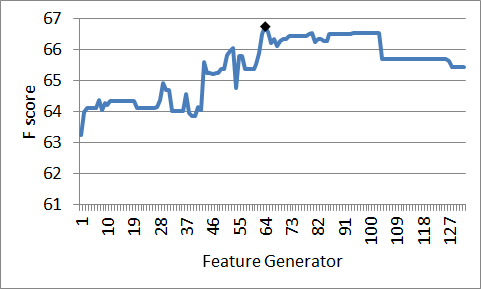
\includegraphics[width=.95\textwidth]{figures/DSAvgAnalysis.png}
  \caption{Average analysis results.}
  \label{fig:DS_AvgAnalysis}
\end{minipage}%
\begin{minipage}{.5\textwidth}
  \centering
  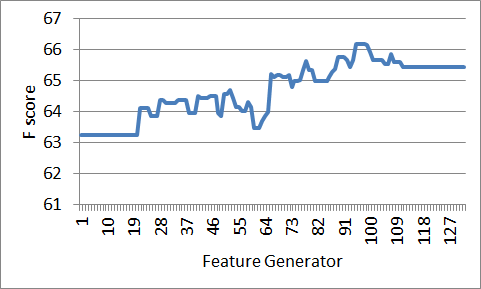
\includegraphics[width=.95\textwidth]{figures/DSMinAnalysis.png}
  \caption{Min IG analysis results.}
  \label{fig:DS_MinAnalysis}
\end{minipage}
\end{figure}

Figure \ref{fig:DS_AvgAnalysis} shows the results of AvgIG analysis and \ref{fig:DS_MinAnalysis} shows the results of MinIG analysis. As seen in Fig. \ref{fig:DS_AvgAnalysis}, the $Avg_{64}$ model registers the best performance with a \textit{F score} of 66.73. This model also reduces the number of features from 310512 to 92514 for 5 rounds of cross validation (reduction of average number of features per round from 62000 to 18500). Since this model registers the best performance and massively reduces the number of features, this model was considered as the best model from feature selection experiments.

\subsection{Hyperparameter Search Results}

The optimal model $Avg_{64}$ was tested for optimal hyperparameter. Exhaustive hyperparameter search was carried out with hyperparameter ranging from 0.0000 to 2.0000 with the steps of 0.0005. Before the exhaustive searching, the hyperparameter used was 0.0065. After the exhaustive search, the same hyperparameter registered the best performance. Therefore, no change was made for the value of hyperparameter.

\subsection{Final Results}

After rigorous feature selection and hyperparameter search, the optimal \textit{DSModel} was used for evaluation of unseen test data.

\begin{figure}
\centering
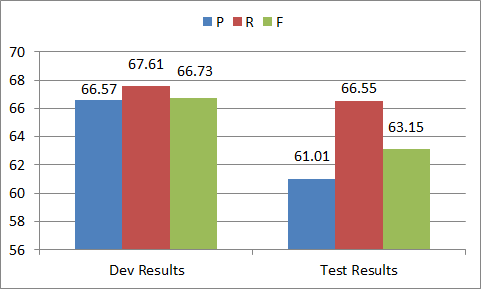
\includegraphics[scale=0.7]{figures/DSFinalResults.png}
\caption{Final evaluation on test set.}\label{fig:DSFinal}
\end{figure}

Figure \ref{fig:DSFinal} shows the comparison between results on development set and test set. The \textit{F score} on development set is 66.73 while that on test set is 63.15.

\section{Initial Results on Full-Text Subcorpus} \label{sec:FTPrimaryRes}

As discussed in Section \ref{sec:full-text}, the full-text subcorpus in LocText consists of 4 PMC \cite{pmc} full-text articles. As the protein-location relations in the full-text subcorpus consists of 92.2\% same-sentence relations (in other words, a mere 7.8\% were different-sentence relations; see Fig. \ref{fig:FT_PLRelDist}), I decided to extract the protein-location relations using the same-sentence model (\textit{SSModel}) only.

\textit{SSModel}, already tuned after thorough experimentation on the abstracts subcorpus, was used directly for extracting relations on full text. Here, none of the tuning experiments, except undersampling \cite{akbani2004applying} of the negative class, were repeated. The original proportion of positive instances to negative instances was 1:5. Different proportions were experimented by using undersampling of negative class and the proportion of 1:1 was found optimal.

\begin{figure}
\centering
\begin{minipage}{.5\textwidth}
  \centering
  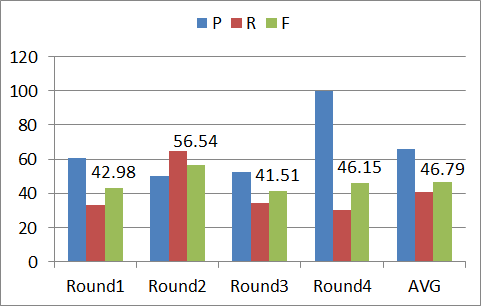
\includegraphics[width=.95\textwidth]{figures/3_FTOrigRatioResults.png}
  \caption{Non unique evaluation results using original proportion.}
  \label{fig:FT_ResOrigNonUniq}
\end{minipage}%
\begin{minipage}{.5\textwidth}
  \centering
  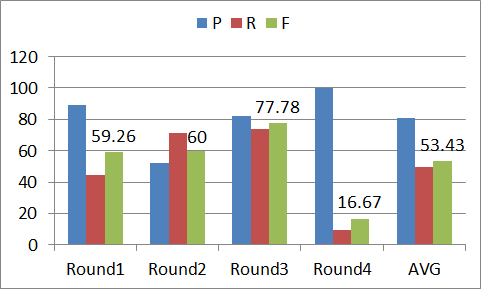
\includegraphics[width=.95\textwidth]{figures/3_FTOrigRatioResults_Uniq.png}
  \caption{Unique evaluation results using original proportion.}
  \label{fig:FT_ResOrigUniq}
\end{minipage}
\end{figure}

4-fold cross validation was used, where every document was used as the total test set once. Thus, in every round of cross validation, the data set was broken down into a training set consisting of 3 documents and test set consisting of a single document. Since there were no tuning experiments to be carried out, a development set was not created.

Fig. \ref{fig:FT_ResOrigNonUniq} and Fig. \ref{fig:FT_ResOrigUniq} shows the evaluation results using the original proportion of positive and negative examples.  Fig. \ref{fig:FT_ResOrigNonUniq} shows the evaluation results using non-unique mode of evaluation and \ref{fig:FT_ResOrigUniq} shows the evaluation results using unique mode of evaluation. The \textit{F scores} bars are labeled in both figures. For non unique mode of evaluation, \textit{SSModel} achieves an average \textit{F score} of 46.79 and for unique mode of evaluation, \textit{SSModel} achieves an average \textit{F score} of 53.43.

%\begin{figure}
%\centering
%\begin{minipage}{.5\textwidth}
%  \centering
%  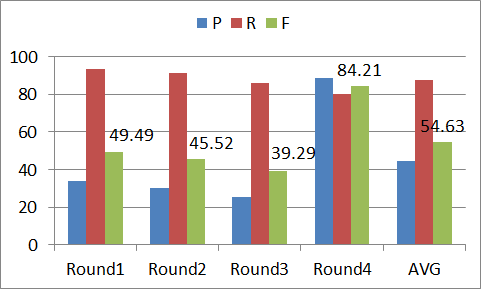
\includegraphics[width=.95\textwidth]{figures/4_FTSameRatioResults.png}
%  \caption{Non unique evaluation results after undersampling negative class}
%  \label{fig:FT_ResUnderSampNonUniq}
%\end{minipage}%
%\begin{minipage}{.5\textwidth}
%  \centering
%  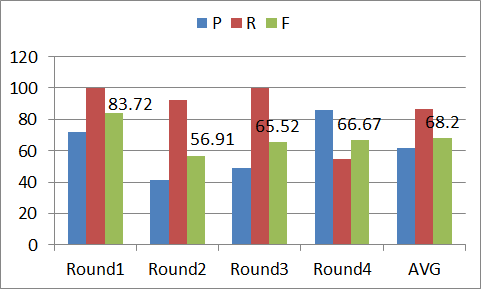
\includegraphics[width=.95\textwidth]{figures/4_FTSameRatioResults_Uniq.png}
%  \caption{Unique evaluation results using after undersampling negative class}
%  \label{fig:FT_ResUnderSampUniq}
%\end{minipage}
%\end{figure}

\begin{figure}
\centering
\begin{subfigure}{.5\textwidth}
  \centering
  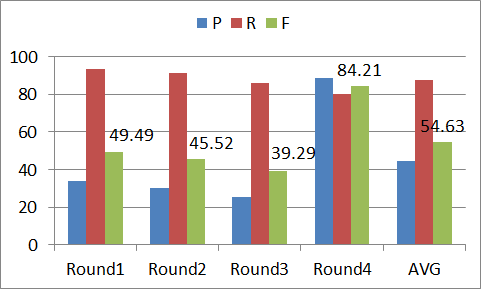
\includegraphics[width=.95\linewidth]{figures/4_FTSameRatioResults.png}
  \caption{Non unique evaluation results.}
  \label{fig:FT_ResUnderSampNonUniq}
\end{subfigure}%
\begin{subfigure}{.5\textwidth}
  \centering
  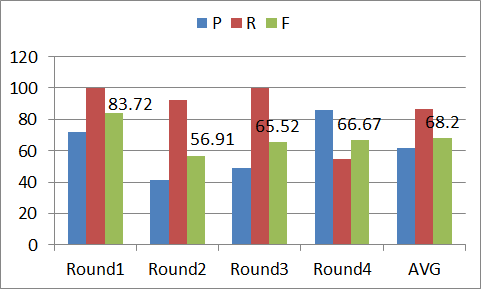
\includegraphics[width=.95\linewidth]{figures/4_FTSameRatioResults_Uniq.png}
  \caption{Unique evaluation results.}
  \label{fig:FT_ResUnderSampUniq}
\end{subfigure}
\caption{Evaluation results after undersampling negative class.}
%\label{fig:test}
\end{figure}

As stated earlier, a proportion of 1:1 was found to be optimal. A proportion of 1:1 implies that the negative class was undersampled to such an extent that the number of negative examples becomes equal to the number of positive examples. Fig. \ref{fig:FT_ResUnderSampNonUniq} shows the results of non unique evaluation using 1:1 proportion and Fig. \ref{fig:FT_ResUnderSampUniq} shows the results of unique evaluation using 1:1 proportion. \textit{SSModel} achieves an average \textit{F score} of 54.63 for non unique evaluation mode and 68.2 for unique evaluation mode. The unique \textit{F score} of 68.2 is better than the best \textit{F score} achieved on the abstracts corpus, namely, 63.15 on test set (Fig. \ref{fig:DSFinal}). However, these are preliminary results and there is a need of experimenting with more data as well as tuning the model specifically to full text.


%\section{Results for CombinedModel}

%\section{Assessment of Performance evaluation results}

%  Explain about statistical significance tests